\chapter{فصل مكونات الخلائط}\label{ch:g3:separating-mixtures}

بعد العاصفة تصير برك الطريق بنية: ماء مطر مختلط بالتراب والرمل وقطع
الأوراق. ومع ذلك فالماء الذي يخرج من صنبور المطبخ رائق، وقد كان هو
أيضًا مطرًا يومًا ما، قبل أن يجري إلى النهر. فكيف يعود الماء الموحل
نظيفًا؟ الأشياء التي خُلطت يمكن أن تُفصل. ويبيّن هذا الفصل كيف، طريقةً
بعد طريقة.

\begin{recall}
\omterm{def:g2:mixing-and-dissolving:mix}{الخلط} أن نضع أشياء مختلفة معًا. والجسم الصلب مثل السكر أو الملح \omterm{def:g2:mixing-and-dissolving:dissolve}{يذوب}
في الماء: يختفي عن العين، والسائل الرائق \omterm{def:g2:mixing-and-dissolving:dissolve}{محلول}. والجسم الصلب الذائب
لا يزال موجودًا: فحين يجف الماء يبقى الجسم الصلب بعده. أما الرمل
والتراب فلا يذوبان
(\cref{ch:g2:mixing-and-dissolving}).
\end{recall}

\section{الفرز باليد والغربلة}

حين تكون قطع الخليط كبيرة بما يكفي لتُرى وتُلتقط، فأبسط طريقة لفصلها
هي اليد: يمكن التقاط حبات الزبيب من الموسلي واحدة واحدة. وحين تكثر
القطع كثيرًا يتولى الغربال الفرز عنا.

\begin{definition}[الغربلة]\label{def:g3:separating-mixtures:sieve}
\emph{الغربلة}\index{غربلة} فصل قطع الخليط بحسب حجمها، بواسطة
غربال: شبكة أو صفيحة مليئة بالثقوب. تسقط القطع الصغيرة من الثقوب،
وتبقى القطع الكبيرة في الغربال.
\end{definition}

\begin{example}[الحصى والرمل]\label{ex:g3:separating-mixtures:gravel}
يهز عامل بناء خليطًا من الحصى والرمل فوق غربال. فيسقط الرمل الناعم
عبره في كومة تحته، ويبقى الحصى على الشبكة.
\end{example}

\begin{omfigure}
\begin{tikzpicture}[font=\small]
  % the sieve: a mesh bowl
  \fill[pattern=crosshatch, pattern color=black!45] (-1.6,2.6) arc[start angle=180,
    end angle=360, x radius=1.6, y radius=0.7] -- cycle;
  \draw[black!70, line width=0.8pt] (-1.6,2.6) arc[start angle=180, end angle=360,
    x radius=1.6, y radius=0.7];
  \draw[black!70, line width=0.8pt] (-1.75,2.6) -- (1.75,2.6);
  \draw[black!70, line width=1.4pt] (1.75,2.6) -- (3.0,2.85);
  % gravel kept in the sieve
  \foreach \x/\y/\r in {-0.9/2.25/0.17,-0.45/2.12/0.2,0.05/2.08/0.18,0.5/2.13/0.21,
                        0.95/2.28/0.16,-0.2/2.42/0.15,0.3/2.43/0.17}
    \fill[black!45, draw=black!65] (\x,\y) circle (\r);
  % sand falling
  \foreach \x/\y in {-0.4/1.6,0.1/1.4,0.4/1.7,-0.15/1.15,0.25/1.0,-0.5/0.95,0.0/0.75}
    \fill[orange!60!brown] (\x,\y) circle (0.05);
  % the heap of sand in a bowl
  \fill[orange!45!brown!70] (-1.0,0.12) .. controls (-0.5,0.55) and (0.5,0.55)
    .. (1.0,0.12) -- cycle;
  \draw[black!70, line width=0.8pt] (-1.5,0.5) .. controls (-1.3,0) and (1.3,0)
    .. (1.5,0.5);
  \node[anchor=west] at (2.0,2.2) {يبقى الحصى في الغربال};
  \node[anchor=west] at (2.0,1.25) {يسقط الرمل من الثقوب};
  \node[anchor=west] at (2.0,0.3) {كومة من الرمل};
\end{tikzpicture}

{\small \omterm{def:g3:separating-mixtures:sieve}{غربلة} خليط من الحصى والرمل: تُفرز القطع بحسب
حجمها.}
\end{omfigure}

\begin{omfigure}
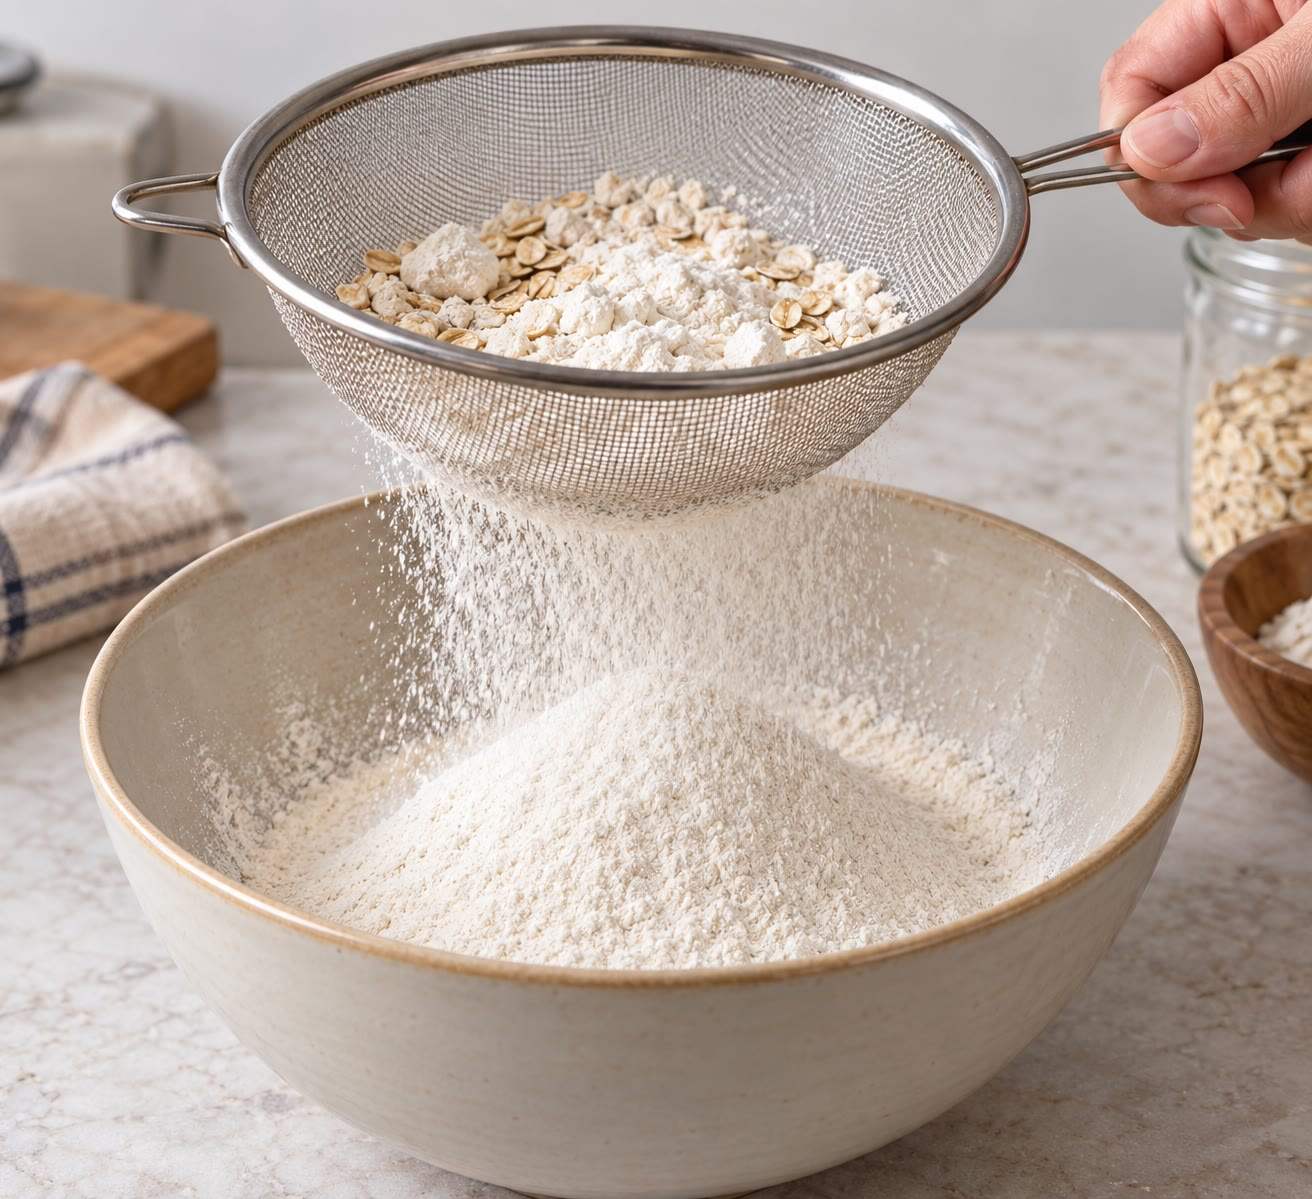
\includegraphics[width=0.55\linewidth]{images/book1/ai/g3-kitchen-sieve.jpg}

{\small غربال المطبخ: يمر الدقيق الناعم، وتبقى الكتل
فيه.}
\end{omfigure}

\section{الترسيب والترويق}

\begin{definition}[الترسيب والترويق]\label{def:g3:separating-mixtures:decant}
يمكن أن نترك ساكنًا خليطًا من الماء وجسم صلب لا \omterm{def:g2:mixing-and-dissolving:dissolve}{يذوب} فيه: فينزل الجسم
الصلب ببطء إلى القاع. ويسمى هذا \emph{الترسيب}\index{ترسيب}.
وبعد أن يترسب الجسم الصلب يمكن أن نصب الماء الرائق الذي فوقه برفق في
وعاء آخر، ونترك الجسم الصلب في مكانه: وهذا هو
\emph{الترويق}\index{ترويق}.
\end{definition}

\begin{omfigure}
\begin{tikzpicture}[font=\small]
  % 1: stirred, cloudy
  \pic at (0,0) {beaker={0.7}{brown!28}};
  \foreach \x/\y in {-0.5/0.3,-0.2/0.6,0.3/0.4,0.5/0.9,-0.4/1.0,0.1/1.2,0.4/0.15,
                     -0.1/0.25,0.2/0.8,-0.55/0.7}
    \fill[brown!60] (\x,\y) circle (0.03);
  \node[anchor=north, align=center] at (0,-0.15) {بعد التحريك:\\ عكر};
  \draw[->, thick, omProp] (1.1,1.0) -- (2.4,1.0);
  % 2: settled
  \pic at (3.5,0) {beaker={0.7}{omWater!80}};
  \fill[brown!60] (2.7,0) rectangle (4.3,0.25);
  \draw[omGlass, line width=0.7pt] (2.7,0.25) -- (2.7,0) -- (4.3,0) -- (4.3,0.25);
  \node[anchor=north, align=center] at (3.5,-0.15) {بعد تركه ساكنًا:\\ ترسب التراب};
  \draw[->, thick, omProp] (4.6,1.0) -- (5.9,1.0);
  % 3: decanted
  \pic at (7.0,0) {beaker={0.1}{omWater!80}};
  \fill[brown!60] (6.2,0) rectangle (7.8,0.25);
  \draw[omGlass, line width=0.7pt] (6.2,0.25) -- (6.2,0) -- (7.8,0) -- (7.8,0.25);
  \pic at (9.2,0) {beaker={0.58}{omWater!80}};
  \node[anchor=north, align=center] at (8.1,-0.15) {بعد الصب: الماء الرائق\\ على اليمين، والتراب باقٍ};
\end{tikzpicture}

{\small ترسيب خليط من التراب والماء، ثم ترويقه.}
\end{omfigure}

\begin{remark}[الترسيب يحتاج إلى وقت]\label{rem:g3:separating-mixtures:time}
الحبيبات الكبيرة الثقيلة تترسب في بضع دقائق؛ أما الطين الناعم جدًا فقد
يحتاج إلى يوم أو أكثر، ويبقى الماء خلال ذلك عكرًا قليلًا. ولا يزيل
\omterm{def:g3:separating-mixtures:decant}{الترويق} كل حبة أبدًا: فقليل من العكارة ينصب مع الماء.
\end{remark}

\section{الترشيح}

\begin{definition}[الترشيح والراشح]\label{def:g3:separating-mixtures:filter}
\emph{الترشيح}\index{ترشيح} صب الخليط عبر مرشِّح: ورقة، أو قطعة
قماش، أو طبقة من الرمل، ثقوبها أصغر من أن تمر منها القطع الصلبة.
يبقى الجسم الصلب على المرشِّح؛ ويسمى السائل الرائق الذي يمر عبره
\emph{الراشح}\index{راشح}.
\end{definition}

\begin{omfigure}
\begin{tikzpicture}[font=\small, scale=1.4]
  \pic[transform shape] at (0,0) {beaker={0.35}{omWater!80}};
  \pic[transform shape] at (0,1.4) {funnel={brown!55}};
  % muddy water waiting in the paper cone, above the soil
  \fill[brown!25] (-0.411,2.45) -- (0.411,2.45) -- (0.722,2.8) -- (-0.722,2.8) -- cycle;
  % drops of filtrate
  \foreach \y in {1.15,0.95} \fill[omDef!50] (0,\y) circle (0.04);
  \draw[<-, omProp, thick] (0.75,2.6) -- (2.0,2.9) node[right, text=black]
    {ورق ترشيح في قمع};
  \draw[<-, omProp, thick] (0.25,2.15) -- (2.0,2.2) node[right, text=black]
    {يبقى التراب على الورق};
  \draw[<-, omProp, thick] (0.85,0.4) -- (2.0,0.6) node[right, text=black]
    {الراشح: ماء رائق};
\end{tikzpicture}

{\small \omterm{def:g3:separating-mixtures:filter}{ترشيح} الماء الموحل عبر ورق \omterm{def:g3:separating-mixtures:filter}{ترشيح}.}
\end{omfigure}

\begin{inthelab}[ترشيح الماء الموحل]
يطوي المعلم ورقة \omterm{def:g3:separating-mixtures:filter}{ترشيح} مستديرة على شكل مخروط ويضعها في قمع زجاجي فوق
كأس. ثم يصب الماء الموحل في المخروط شيئًا فشيئًا، ولا يتجاوز به حافة
الورقة أبدًا. فيقطر الماء الرائق في الكأس، ويكوّن التراب طبقة بنية على
الورقة. وإذا كان \omterm{def:g3:separating-mixtures:filter}{الراشح} عكرًا فالورقة ممزقة أو أن الماء تجاوز حافتها.
\end{inthelab}

\begin{proposition}[المرشِّح لا يحجز ما هو ذائب]\label{prop:g3:separating-mixtures:dissolved}
يحجز المرشِّح القطع الصلبة غير الذائبة. ولا يحجز ما هو ذائب: فالماء
المالح الذي يُصب عبر مرشِّح يخرج مالحًا كما كان، والشاي المحلّى يخرج
حلوًا كما كان.
\end{proposition}

\begin{omfigure}
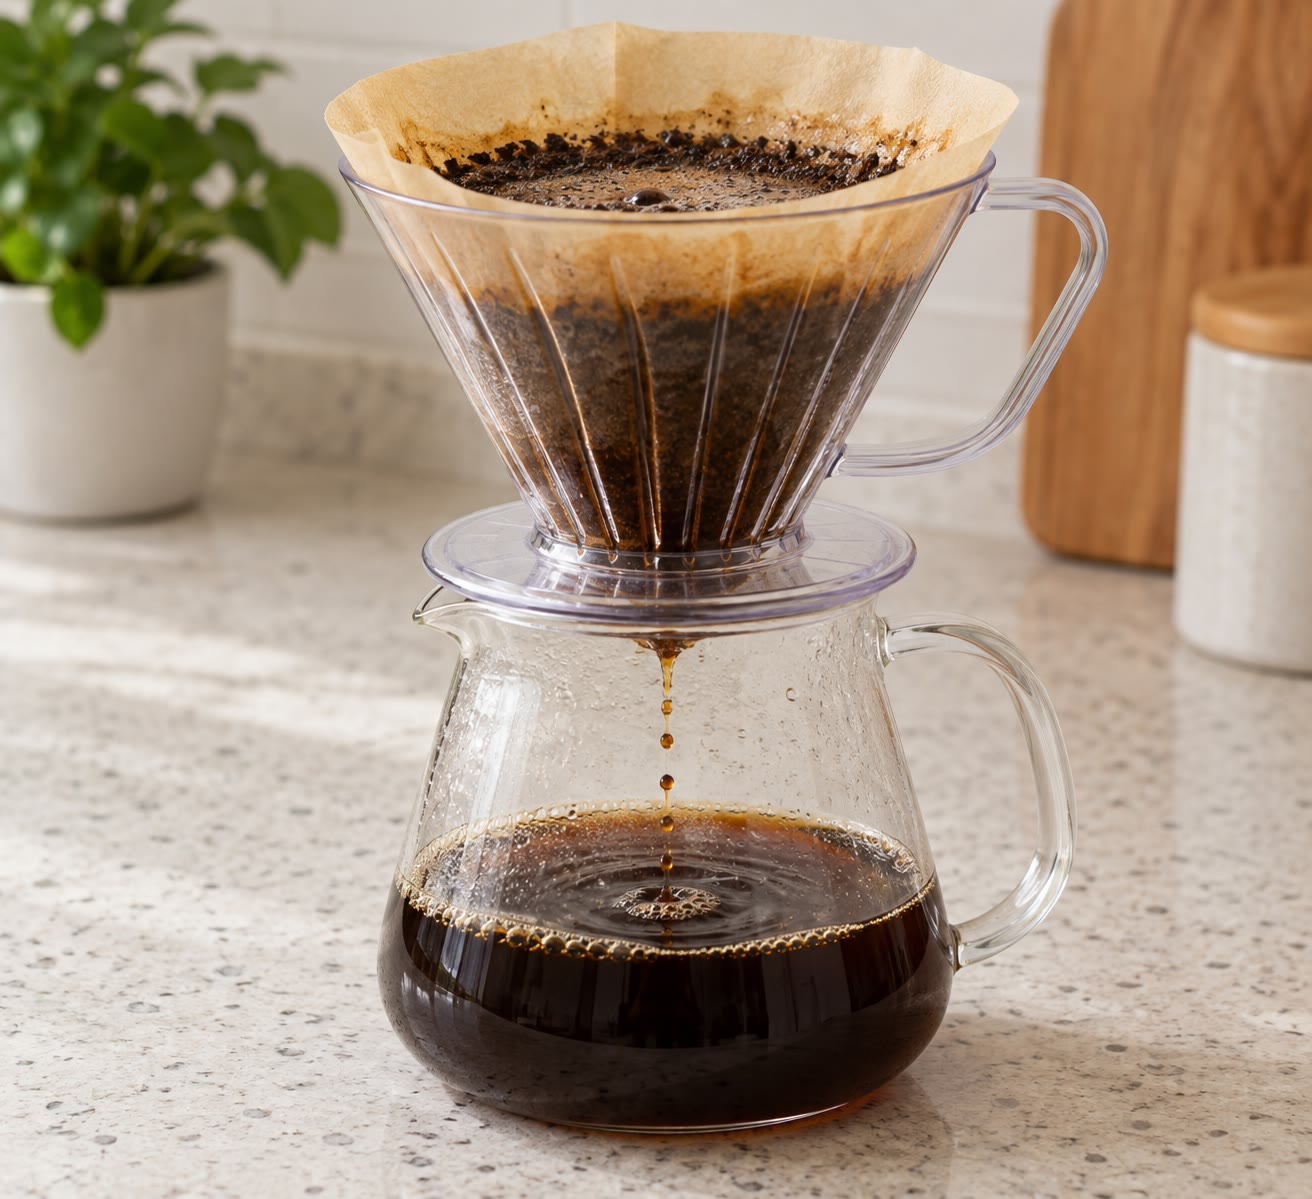
\includegraphics[width=0.5\linewidth]{images/book1/ai/g3-coffee-filter.jpg}

{\small تحضير القهوة \omterm{def:g3:separating-mixtures:filter}{ترشيح}: يبقى البن المطحون في الورقة، والقهوة هي
\omterm{def:g3:separating-mixtures:filter}{الراشح}.}
\end{omfigure}

\section{تبخير الماء}

\begin{definition}[التبخير]\label{def:g3:separating-mixtures:evaporate}
لاسترجاع جسم صلب ذائب في الماء نترك الماء يجف، في الشمس أو على حرارة
هادئة: وهذا هو \emph{التبخير}\index{تبخير}. يذهب الماء إلى
الهواء، ويبقى الجسم الصلب في الصحن.
\end{definition}

\begin{example}[الملح من الماء المالح]\label{ex:g3:separating-mixtures:salt}
نصب قليلًا من الماء المالح في صحن قليل العمق ونتركه على حافة نافذة
مشمسة. وبعد أيام لا يبقى ماء، بل قشرة بيضاء من الملح فقط: إنه الملح
الذي كان ذائبًا.
\end{example}

\begin{omfigure}
\begin{tikzpicture}[font=\small, scale=1.4]
  \pic[transform shape] at (0,0) {hotplate};
  \pic[transform shape] at (0,0) {evapdish={omWater!80}};
  \node[anchor=north, align=center] at (0,-0.6) {ماء مالح\\ يُسخَّن بهدوء};
  \draw[->, thick, omProp] (1.5,0.3) -- (3.0,0.3) node[midway, above, text=black]
    {لاحقًا};
  \pic[transform shape] at (4.5,0) {hotplate};
  \pic[transform shape] at (4.5,0) {evapdish={white!85!black}};
  \foreach \x in {-0.45,-0.25,-0.05,0.15,0.35}
    \fill[white, draw=black!45, line width=0.2pt] (4.5+\x,0.12) rectangle ++(0.09,0.06);
  \node[anchor=north, align=center] at (4.5,-0.6) {لم يبقَ ماء:\\ بلورات الملح};
  \foreach \x in {-0.3,0,0.3} \draw[->, black!45, decorate,
    decoration={snake, amplitude=0.6pt, segment length=4pt}] (\x,0.7) -- (\x,1.4);
  \node[anchor=south] at (0,1.4) {يذهب الماء إلى الهواء};
\end{tikzpicture}

{\small \omterm{def:g3:separating-mixtures:evaporate}{التبخير} في المختبر: يسخّن المعلم الصحن بهدوء على صفيحة
تسخين. ويبقى الملح في الصحن.}
\end{omfigure}

\section{أي طريقة لأي خليط؟}

\begin{method}[اختيار طريقة الفصل]\label{met:g3:separating-mixtures:choose}
لتفصل مكونات خليط، اسأل:
\begin{enumerate}
  \item هل القطع كبيرة ومختلفة الأحجام؟ افرز باليد، أو
        غربل.
  \item هل في السائل جسم صلب لا \omterm{def:g2:mixing-and-dissolving:dissolve}{يذوب}؟ اتركه يترسب ثم روّق، أو
        رشّح لتحصل على ماء أصفى.
  \item هل في السائل جسم صلب ذائب؟ بخّر السائل:
        فيبقى الجسم الصلب.
\end{enumerate}
وكثيرًا ما نحتاج إلى عدة خطوات، واحدة بعد أخرى.
\end{method}

\begin{example}[الرمل والملح والماء]\label{ex:g3:separating-mixtures:three}
في مرطبان ماء فيه رمل وملح. ذاب الملح، ولم يذب
الرمل.
\begin{enumerate}
  \item رشّح: يبقى الرمل على الورقة.
  \item \omterm{def:g3:separating-mixtures:filter}{الراشح} رائق، لكنه ماء مالح. بخّره: فيبقى
        الملح في الصحن.
\end{enumerate}
طريقتان، واحدة بعد الأخرى، تعيدان إلينا الرمل والملح.
\end{example}

\begin{example}[ماء نظيف من النهر]\label{ex:g3:separating-mixtures:plant}
تجعل محطة معالجة المياه ماء النهر صالحًا للشرب في عدة خطوات:
\begin{enumerate}
  \item يمر ماء النهر عبر مصافٍ، وهي شبكات كبيرة توقف
        الأغصان والأوراق والبلاستيك: وهذا نوع من \omterm{def:g3:separating-mixtures:sieve}{الغربلة}؛
  \item يسكن في أحواض كبيرة يترسب فيها الطين في القاع؛
  \item يُرشَّح عبر طبقات سميكة من الرمل تحجز أدق
        الحبيبات؛
  \item يضاف إليه مقدار ضئيل جدًا من مادة تقتل الجراثيم، كي
        يبقى الماء آمنًا في الأنابيب.
\end{enumerate}
\end{example}

\begin{omfigure}
\begin{tikzpicture}[font=\small, node distance=0.45cm,
    box/.style={draw=omDef, fill=omDef!6, rounded corners=2pt, align=center,
      minimum height=1.15cm, text width=2.0cm}]
  \node[box] (r) {ماء\\ النهر};
  \node[box, right=of r] (s) {المصافي\\ (غربلة)};
  \node[box, right=of s] (t) {أحواض\\ الترسيب};
  \node[box, right=of t] (f) {مرشِّحات\\ الرمل};
  \node[box, right=of f] (g) {قتل\\ الجراثيم};
  \foreach \a/\b in {r/s,s/t,t/f,f/g} \draw[->, thick, omProp] (\a) -- (\b);
  \node[below=0.15cm of s, font=\footnotesize, align=center] {أغصان،\\ بلاستيك};
  \node[below=0.15cm of t, font=\footnotesize, align=center] {الطين};
  \node[below=0.15cm of f, font=\footnotesize, align=center] {حبيبات دقيقة};
  \draw[->, thick, omProp] (g.south) -- ++(0,-0.8) node[below] {إلى الصنابير};
\end{tikzpicture}

{\small مراحل محطة معالجة المياه. تحت كل مرحلة: ما
تزيله.}
\end{omfigure}

\begin{omfigure}
\begin{minipage}[t]{0.48\linewidth}\centering
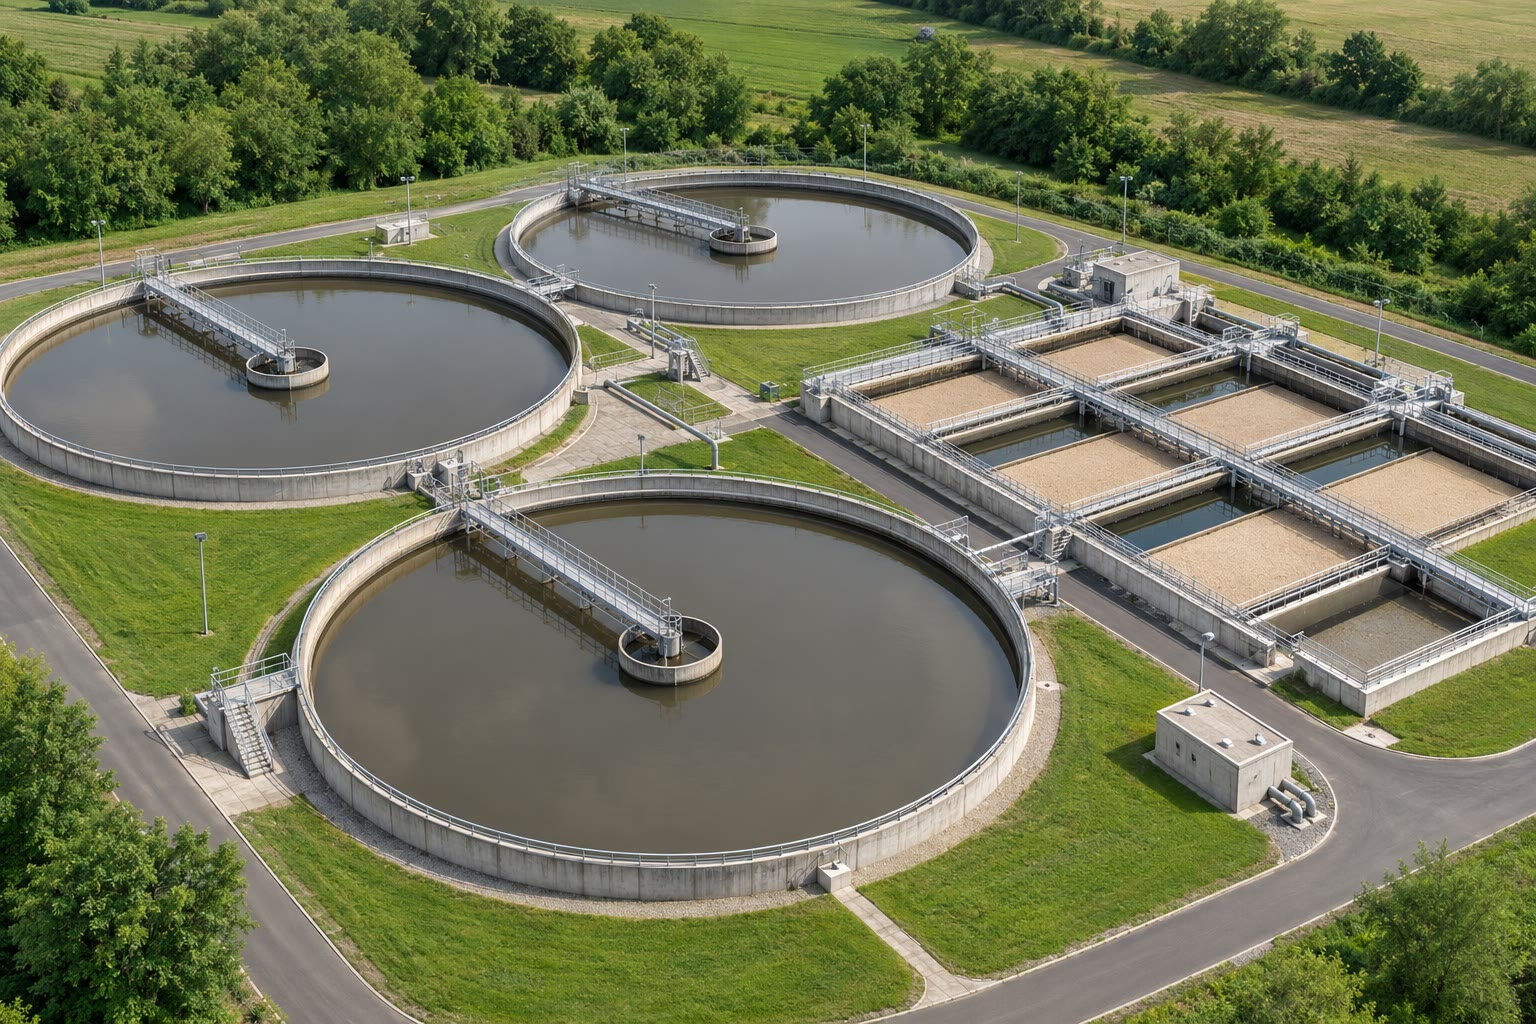
\includegraphics[width=\linewidth,height=4.6cm,keepaspectratio]{images/book1/ai/g3-settling-tanks.jpg}

{\small أحواض الترسيب في محطة لمعالجة المياه.}
\end{minipage}\hfill
\begin{minipage}[t]{0.48\linewidth}\centering
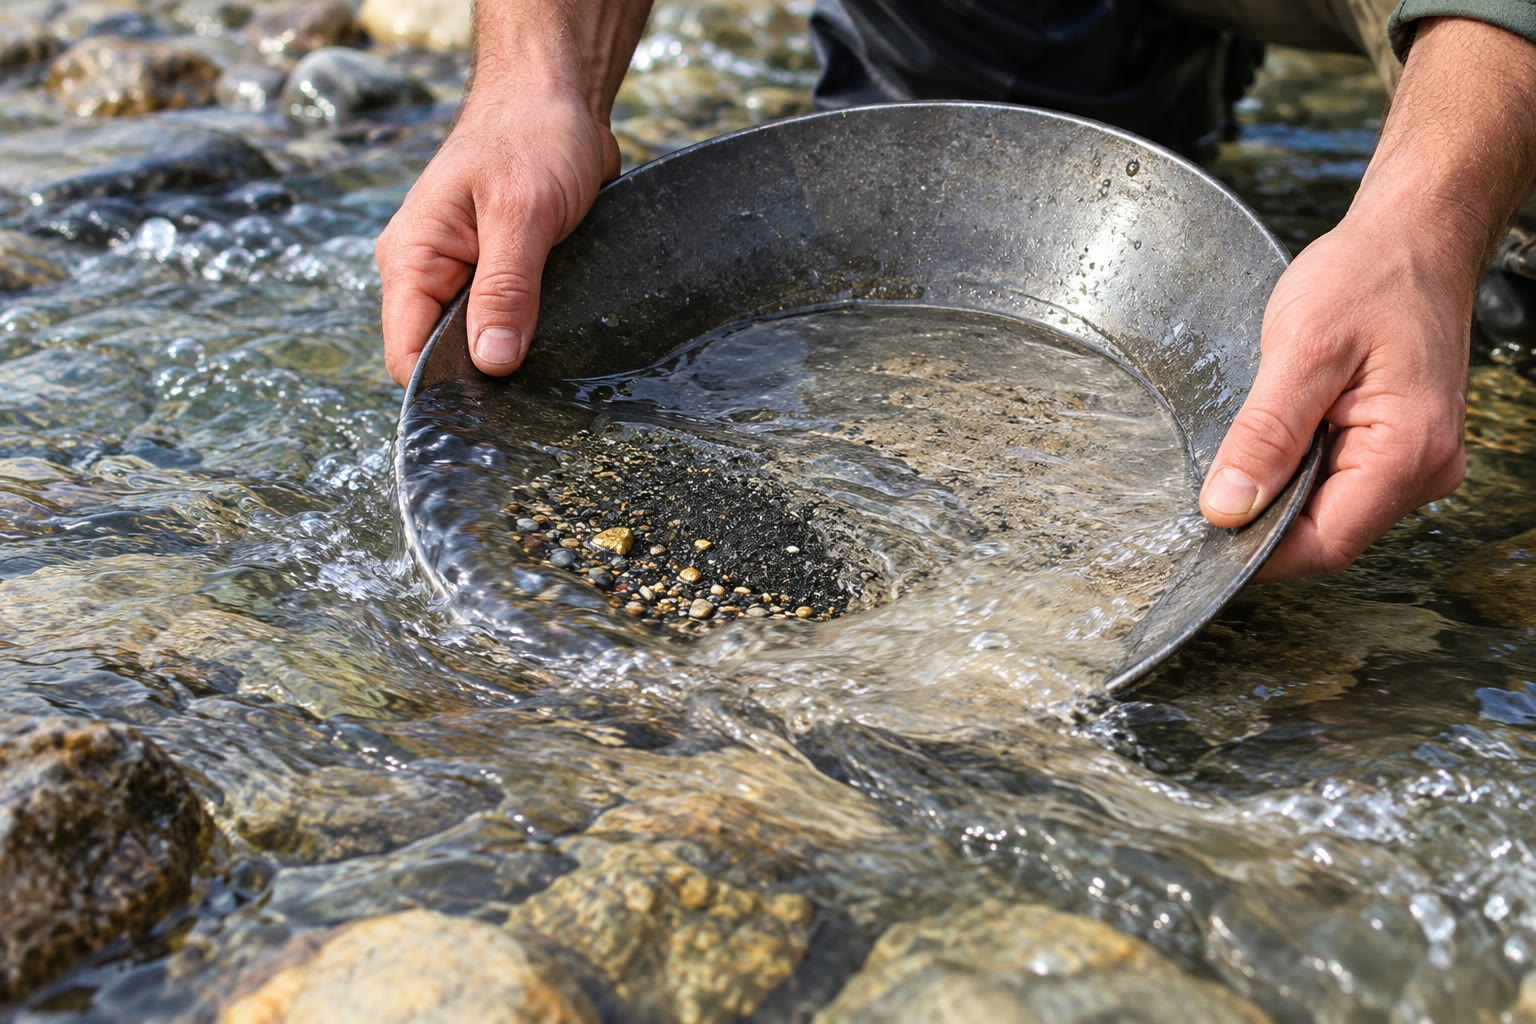
\includegraphics[width=\linewidth,height=4.6cm,keepaspectratio]{images/book1/ai/g3-gold-panning.jpg}

{\small التنقيب عن الذهب: يحمل ماء النهر الرمل الخفيف بعيدًا،
وتبقى الحبيبات الثقيلة في الصحن.}
\end{minipage}
\end{omfigure}

\begin{remark}[الرائق ليس دائمًا نظيفًا]\label{rem:g3:separating-mixtures:clean}
قد يبدو الماء المرشَّح رائقًا تمامًا ومع ذلك يحوي مواد ذائبة، وجراثيم
أصغر بكثير من أن تُرى. ولهذا لا يشرب أحد ماء بركة أو جدول، حتى بعد
ترشيحه.
\end{remark}

\section{تمارين}

\begin{exercise}[$\star$]\label{exo:g3:separating-mixtures:1}
أي طريقة تستعمل لفصل حبات البازلاء عن حبات الأرز؟
\end{exercise}

\begin{exercise}[$\star$]\label{exo:g3:separating-mixtures:2}
تُترك كأس ماء موحل على طاولة ساعة كاملة. ماذا يحدث للتراب؟ وماذا
يسمى ذلك؟
\end{exercise}

\begin{exercise}[$\star$]\label{exo:g3:separating-mixtures:3}
ما \omterm{def:g3:separating-mixtures:filter}{الراشح}؟ وما \omterm{def:g3:separating-mixtures:filter}{الراشح} حين نحضّر القهوة؟
\end{exercise}

\begin{exercise}[$\star$]\label{exo:g3:separating-mixtures:4}
يُصب ماء مالح عبر ورقة \omterm{def:g3:separating-mixtures:filter}{ترشيح}. هل \omterm{def:g3:separating-mixtures:filter}{الراشح} مالح؟
علّل.
\end{exercise}

\begin{exercise}[$\star$]\label{exo:g3:separating-mixtures:5}
كيف نسترجع السكر من كأس ماء محلّى بالسكر؟
\end{exercise}

\begin{exercise}[$\star$]\label{exo:g3:separating-mixtures:6}
انظر إلى شكل الغربال. أي القطع تبقى في الغربال؟ ولماذا تسقط القطع
الأخرى عبره؟
\end{exercise}

\begin{exercise}[$\star$]\label{exo:g3:separating-mixtures:7}
اربط كل خليط بطريقة --- \omterm{def:g3:separating-mixtures:sieve}{الغربلة} أو \omterm{def:g3:separating-mixtures:filter}{الترشيح} أو \omterm{def:g3:separating-mixtures:evaporate}{التبخير}:
(أ) رمل وحصى؛ (ب) مسحوق الطباشير في الماء؛ (ج) ملح في الماء.
\end{exercise}

\begin{exercise}[$\star$]\label{exo:g3:separating-mixtures:8}
انظر إلى شكل محطة معالجة المياه. بكم مرحلة يمر الماء؟ وأي مرحلة تزيل
الطين؟
\end{exercise}

\begin{exercise}[$\star$]\label{exo:g3:separating-mixtures:9}
رتّب هذه الخطوات لاسترجاع الرمل والملح من مرطبان فيه رمل وملح وماء:
بخّر \omterm{def:g3:separating-mixtures:filter}{الراشح}؛ رشّح؛ اجمع الرمل من على
الورقة.
\end{exercise}

\begin{exercise}[$\star\star$]\label{exo:g3:separating-mixtures:10}
هل يستطيع مرشِّح أن يجعل ماء البحر صالحًا للشرب؟ علّل لماذا لا.
\end{exercise}

\begin{exercise}[$\star\star$]\label{exo:g3:separating-mixtures:11}
تُركت أوراق الشاي في إبريق مليء بالشاي. سمِّ طريقتين، مما رأيت في هذا
الفصل، تفصلان الشاي عن الأوراق.
\end{exercise}
